%\graphicspath{{./plots/}}


\section{Experimental Setup}
\label{sec:experimnt_setup}

\paragraph{} We conducted sophisticated experiments in which samples were loaded under triaxial conditions inside a pressure vessel and fractured in-situ to simultaneous measure flow rate and elastic properties. Westerly granite samples were prepared by cutting them into L-shape blocks (69 x 45 50 x 26 mm, Figure \ref{fig:samplesetup}) with 3 mm deep notches on the top and bottom to ensure reproducibility of planar fracture propagation. The L-shape is used for maintaining constant nominal contact area during fracture and shear. The samples were saturated in deionized water and then placed between steel forcing blocks that have embedded piezoelectric transducers. The P-polarized lead-zirconate transducers (PZTs) of company APC International Ltd. are 6.5 mm in diameter, with a center frequency of 500 kHz and the spacing between the steel loading platen and the PZTs is 4mm. The shorter forcing block additionally contains internal conduits to provide fluid flow along the fracture plane. Deionized water was pumped through these narrow channels (45 x 1 mm) and covered by sintered porous fits and fed by five 1.6 mm diameter holes. Sintered porous frits (permeability ~ $10^{-14}$ $m^2$) are press-fit into cavities within the short forcing block to allow homogenous distribution of fluid. After securing this Single Direct Shear (SDS) configuration, it was sealed inside a latex jacket to separate confining and pore fluids. Fully prepared and jacketed samples were fitted inside a pressure vessel within a biaxial loading apparatus.

\paragraph{} The Biax consists of two hydraulic pistons capable of applying vertical and horizontal loads in displacement or load control. Forces are measured using custom-built, beryllium-copper strain-gauge load cells mounted on each loading piston. The load cells have an amplified output of ±5 V with an accuracy of ±5 N and are calibrated with a Morehouse proving-ring. Displacements are measured with direct-current displacement transducers (DCDT), with an accuracy of $\pm$ 0.1 $\mu m$. The confining fluid, a food-grade heat transfer oil (XCELTHERM 600, Radco Industries), in the sealed pressure vessel is pressurized to create a true-triaxial stress conditions. A linear variable differential transformer was attached to the outside of the sample, inside the pressure vessel, to accurately ($\pm 0.1\ \mu m$) measure the fracture displacement. Pressure intensifiers fitted with LVDTs and pressure transducers were used to control the confining pressure and the internal upstream and downstream pressures. 

\paragraph{} Each axis of loading is independently servo-controlled and all stresses, strains, fluid pressures and fluid volumes were recorded with $\pm10$ V, 16-channel 24-bit analog-to-digital converter at 10 kHz and averaged to sampling rates of 100 Hz or 1 kHz. Fracture permeability was measured using upstream and downstream pore-pressure intensifiers. Active ultrasonic data were recorded using a Vantage\textsuperscript{TM}\ Research Ultrasound (Verasonics) system. We use broadband (~0.02-2 MHz) PZTs (APC International Ltd. 6.35 diameter compressional crystals), which were successively pulsed every 1 ms on the transmitting side and the recording rate at the receiver side was 25 MHz. The input signal is a half sine with a frequency of 500 kHz. Also, a pulse from the Verasonics system accompanied the PZT excitation and is recorded by the 24-bit analog-to-digital data acquisition system. This allows us to sync the “ultrasonic” to “poro-mechanical” data and then analyzed to measure changes in the permeability and elasticity of the fractured rock samples, explained more fully in the signal analysis procedure.
  
\paragraph{} Before commencing each experiment, the samples were installed in the pressure vessel and then the vessel was sealed and then filled with confining fluid. A horizontal load of 20 MPa was applied and then the confining fluid pressure was slowly increased to 15 MPa; it is important to monitor the integrity sample jacket seal during this step. Next, we applied a pore pressure differential: inlet ($P_{pA}$ = 4 MPa) and outlet ($P_{pB}$ = 2 MPa). At this point there was no flow because Westerly granite matrix permeability is very low ($< 10^{-20}\ m^2$) and the confining fluid pressure is greater than the pore pressure (there was no flow around the sample). After establishing all loads and pore pressure, the ultrasonic data acquisition Once all fluid pressures and solid stresses were applied, the ultrasonic data acquisition system (Verasonics\textsuperscript{\textregistered}) was started. The sample was then fractured in situ by increasing the shear stress at constant normal stress while making continuous measurements of fluid flow and ultrasonic properties. After locking the vertical piston (no displacement allowed), we executed the dynamic stressing protocol illustrated in Figure 2a.

\paragraph{} After executing the normal stress and pore pressure oscillation protocol, the fractured sample was sheared twice in 4 mm increments (for a total of 8 mm). During the shearing phases of the experiment acoustic emissions (AEs) were monitored (passive source recording). Subsequent to shearing the dynamic stressing protocol was repeated. We incorporate shearing in this investigation to determine its influence on the nonlinearity measurements of the fracture. The fracture aperture is changed through shear, in effect, modeling the complexity of fractured subsurface rock. 

\newpage

\begin{figure*}[ht] 
	% read manual to see what [ht] means and for other possible options
	\centering 
	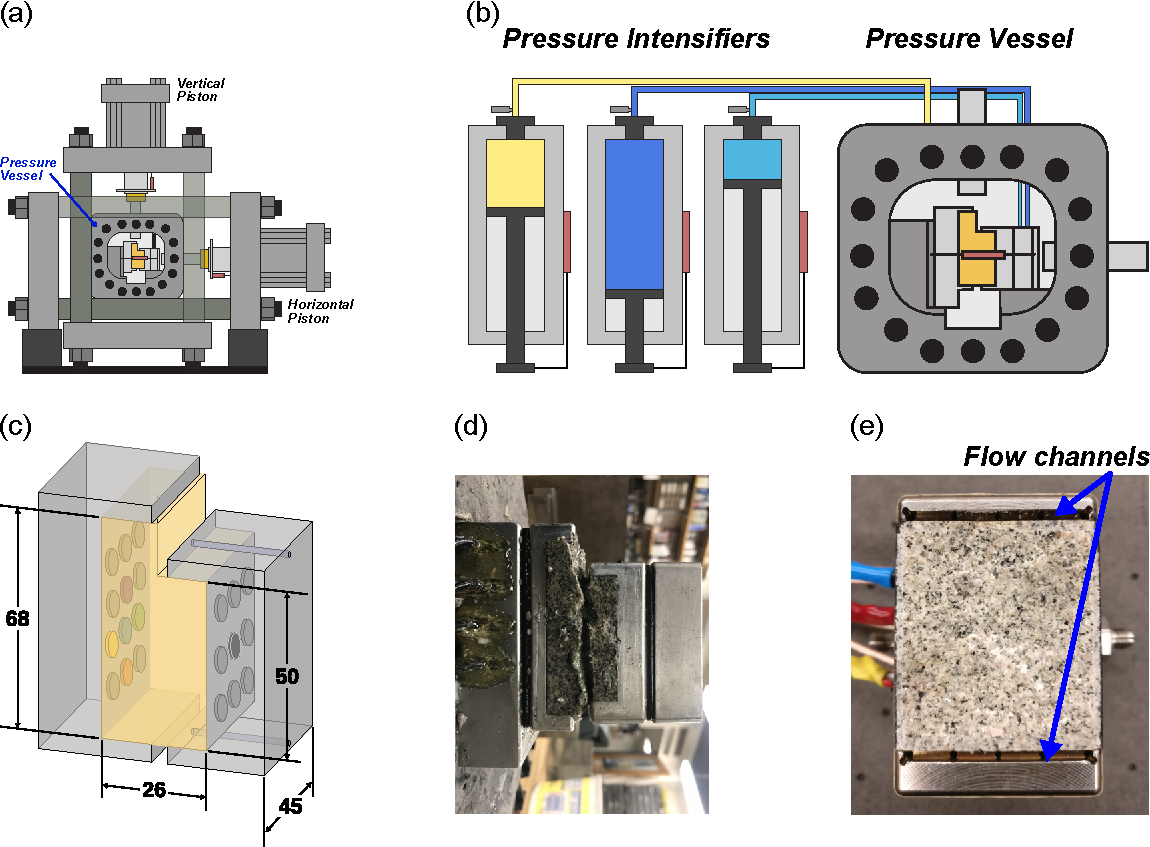
\includegraphics[width=0.9 \columnwidth]{experimental_configuration}
	\caption[]{(a) The experiments were conducted in the Penn State Rock and Sediment Mechanics laboratory using the Biaxial Deformation Apparatus (Biax). The Biax has servo-controlled vertical and horizontal pistons and a 10 kHz 24-bit analog to digital data recorder. (b) A pressure vessel was inserted in the Biax and connected to the pressure intensifiers, which control the confining ($P_C$), and sample ($P_{PA}$ and $P_{PB}$ ) fluid pressures. (c) The Westerly granite sample is machine cut into a L-shape and placed between the two loading platens. These loading platens are embedded with piezoelectric transducers (p-polarized) and contain fluid ports for the inlet and outlet flow. The shorter forcing block additionally contains internal conduits to provide fluid flow along the fracture plane. Deionized water was pumped through these narrow channels (45 x 1 mm) and covered by sintered porous fits and fed by five 1.6 mm diameter holes. Sintered porous frits (permeability $\sim 10^{-14}\ m^2$) are press-fit into cavities within the short forcing block to allow homogeneous distribution of fluid. After securing this Single Direct Shear (SDS) configuration, it was sealed inside a latex jacket to separate confining and pore fluids. (d) A photo of the sample after experimentation highlights the degree of roughness from in-situ fracture. (e) Post mortem sample inside loading block showing the flow channels that feed into the sintered porous frits for fluid distribution along fracture plane. }
	\label{fig:samplesetup} 
\end{figure*}

\newpage

\begin{figure*}[ht]
	\centering
	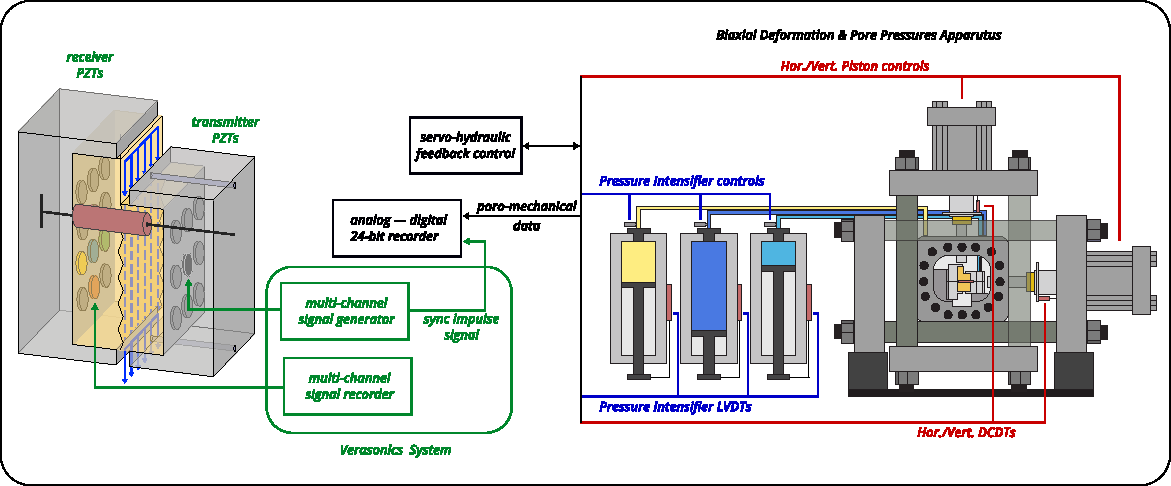
\includegraphics[width=0.9 \columnwidth]{exp_daq_v1}
	\caption[]{Schematic of the single direct shear configuration with the block diagram showing the main features of the data acquisition system for both the poro-mechanical and ultrasonic data. The Biax consists of two hydraulic pistons capable of applying vertical and horizontal loads in displacement or load control. Forces are measured using custom-built, beryllium-copper strain-gauge load cells mounted on each loading piston. The load cells have an amplified output of 5 V with an accuracy of 5 N and are calibrated with a Morehouse proving-ring. Displacements are measured with direct-current displacement transducers (DCDT), with an accuracy of $\pm 0.1 \mu m$. Each axis of loading is independently servo-controlled and all stresses, strains, fluid pressures and fluid volumes were recorded with 10 V, 16-channel 24-bit analog-to-digital converter at 10 kHz and averaged to sampling rates of 100 Hz or 1 kHz. Fracture permeability was measured using upstream and downstream pore-pressure intensifiers. Active ultrasonic data were recorded using a Vantage TM Research Ultrasound (Verasonics) system. We use broadband (0.02-2 MHz) PZTs (APC International Ltd. 6.35 mm diameter compressional crystals), which were successively pulsed every 1 ms on the transmitting side and the recording rate at the receiver side was 25 MHz. The input signal is a half sine with a frequency of 500 kHz. Also, a pulse from the Verasonics system accompanied the PZT excitation and is recorded by the 24-bit analog-to-digital data acquisition system. This allows us to sync the ultrasonic to poro-mechanical data and then analyzed to measure changes in the permeability and elasticity of the fractured rock samples, explained more fully in the signal analysis procedure.}
	\label{fig:data_aq}
\end{figure*}

\newpage


\subsection{Experimental Procedure}
\paragraph{}
Each experiment commenced with extensive sample preparation: in which the Westerly granite was cut and notched, sealed in a latex jacket, and then placed inside the pressure vessel (see Section \ref{sec:experimnt_setup} for details). After sealing the pressure vessel and loading the sample, inlet and outlet flow were pressurized to 4 MPa and 2MPa, respectively. At this stage there was no flow because Westerly granite matrix permeability is very low ($< 10^{-20}\ m^2$ ) and the confining fluid pressure (around the jacketed sample) is much larger than the pore pressure, preventing flow of water around the sample.
A shear load was then applied with the vertical piston in displacement mode at a constant 10 $\mu m/s$, fracturing in-situ after reaching a critical stress of $ \approx $60 MPa, and then locked the vertical piston. During fracture fluid flow and acoustic emissions were measured, but these results are not included in this paper. Next, the dynamic stressing protocol was implemented in which the normal stress and pore pressure were modulated. 
\paragraph{}
Normal stress oscillations were applied by oscillating the horizontal piston of the load frame at prescribed amplitudes (0.2 to 3 MPa) and frequencies (0.1, 1, 10, 40 Hz). Pore pressure oscillations were achieved by oscillating $P_{PA}$ while holding $P_{PB}$ constant at amplitudes of 0.2 to 3 MPa and frequencies of 0.1, 1, 10 Hz. Multiple sets of normal stress and pore pressure oscillations of varying amplitudes and frequencies were applied to investigate: (1) repeatability and direct comparison between the two modulated stresses and (2) amplitude and frequency dependencies of the measured response. Post-fracture dynamic stressing is plotted in Figure \ref{fig:exp_seq}d (highlighted in yellow) and shows the normal stress (red) and pore pressure (blue) oscillations; note that line thickness correlates with oscillation frequency. 
To investigate the effect of fracture aperture on elastic nonlinearity and permeability, the sample was sheared in two 4 mm, (held at $ \sigma_{NS} $ = 20 MPa) stages. After each shearing stage the oscillation protocol was applied to the sample. Initially,the in-situ fracture was quite rough, but the effect of shear reduces and changes this roughness; the old contacts were broken and new contacts formed, changing the extent to which the two halves of the fracture were mated. This allows for investigation of how fracture aperture is related to the elasto-dyamic and hydromechanical properties. 

\newpage


\begin{figure*}[ht]
	\centering
	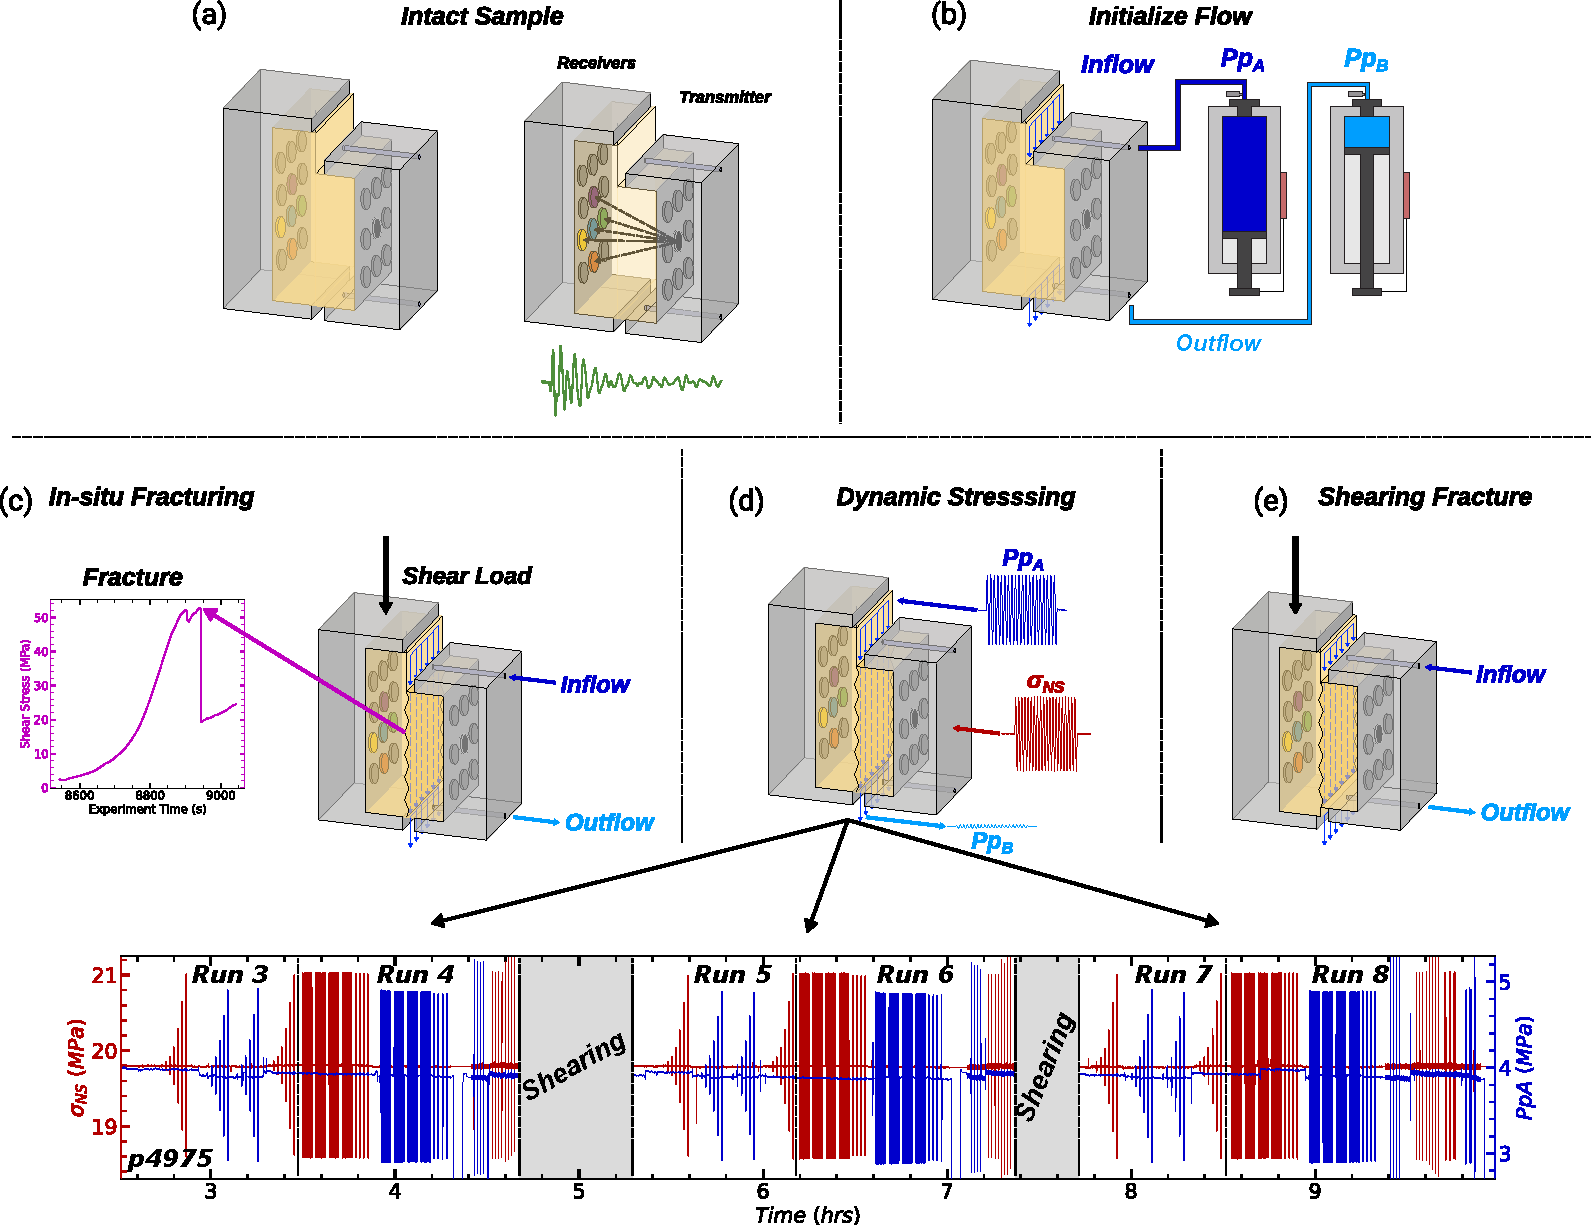
\includegraphics[width=0.99\columnwidth]{exp_sequence_v2}
	\caption[]{(a) Intact Westerly granite sample cartoon, showing dimensions and approximate transmitter - receiver ray paths. 
		(b) Next, we applied a pore pressure differential: inlet ($P_{PA}$ = 4 MPa) and outlet ($P_{PB}$ = 2 MPa). 
		(c) The shear stress was loaded at a constant rate of 10 $\mu m/s$ until reaching the critical shear stress at $ \approx $60 MPa. 
		(d) Cartoon showing the oscillation protocol applied to the freshly fractured sample. Multiple sets of $P_{P}$ and $ \sigma_{NS} $ oscillations of varying amplitude (up to about $ \pm $ 1 MPa) and frequency (0.1, 1, 10 and 40 Hz) were applied. 
		(e) The sample was sheared in two additional increments of 4mm, each followed by the dynamic stressing protocol.}
	\label{fig:exp_seq}
\end{figure*}


\newpage

\subsection{Dynamic Effective Stress Perturbations}
The fractured samples were dynamically perturbed via pore pressure ($P_P$) and normal stress ($\sigma_{n}$) oscillations. Following the procedure described by Candela et al., 2015, pore pressure oscillations were achieved by oscillating $P_{PA}$ while holding $P_{PB}$ constant. Conversely, normal stress oscillations were
applied by oscillating the horizontal piston of the load frame at prescribed amplitude and frequency. 
As depicted in Figure 2a, multiple sets of Pp and $\sigma_n$ oscillations of varying amplitude (up to about $\pm$ MPa) and frequency (0.1, 1, 10 and 40 Hz) were applied to investigate the repeatability as well as amplitude and frequency dependencies of the measured response. Similar parameters were used for $P_P$ and $\sigma_{n}$ oscillation sets in order to apply similar effective stress perturbations and allow making comparisons between $P_P$ and $\sigma_{n}$ stimulations.


\subsection{Permeability Measurements}
\paragraph{} We measured flow rates independently at the inlet ($Q_A$) and outlet ($Q_B$) using the outputs of LVDTs on the pressure intensifiers. After verifying the steady state flow condition ($Q_{A} - Q_{B}  \leq 5 \% $), Darcy’s law was
used to calculate permeability k: 
\begin{equation} \label{eq:perm}
k = \frac{\mu L}{S} \frac{Q}{\Delta P_P}
\end{equation}
where $Q = \frac{1}{2} (Q_A + Q_B )$ is the average flow rate ($\frac{m^3}{s}$), $\mu$ is the fluid viscosity ($10^{-3} Pa\cdot s$) at 20\textdegree\ C, $L$ is the flow path given by the length of the sample (50 mm) and $S$ is the cross section perpendicular to the flow path (45 x 26 $mm^2$).
\paragraph{} Specifically, k is the bulk permeability, that is, the permeability of the surrounding rock matrix (on order of $10^{-21} m^2$) and of the fracture [Zhang et al., 2017; Ishibashi et al., 2018]. Alternative calculations of permeability are valid [Zhang et al., 2017; Ishibashi et al., 2018], however we are interested in relative changes in permeability in response to dynamic stressing, so the absolute value of the permeability is not necessary to quantify.


\subsection{Ultrasonic Measurements: Active Source}
Ultrasonic waves transmitted through the fracture were recorded continuously in each experiment. Half-cycle sinusoidal pulses with an amplitude of 40 V and center frequency of 500 kHz were emitted consecutively from each transmitting transducer (9 piezoelectric discs arranged in a 3 x 3 matrix embedded within the right-hand loading block in Figure 1b) with a pulse repetition frequency (PRF) of 100 Hz or 1000 Hz during the low and high frequency ($\geq 10$ Hz) stress oscillations, respectively. The waveforms were amplified ($\sim 40$ dB) and recorded for all the receiving transducers (12 piezoelectric discs arranged in a 4 x 3 matrix embedded within the left-hand loading block in Figure 1b). We activated up to the full array of 9 transmitter and 12 receivers. 

\newpage

\begin{figure*}[ht]
	\centering
	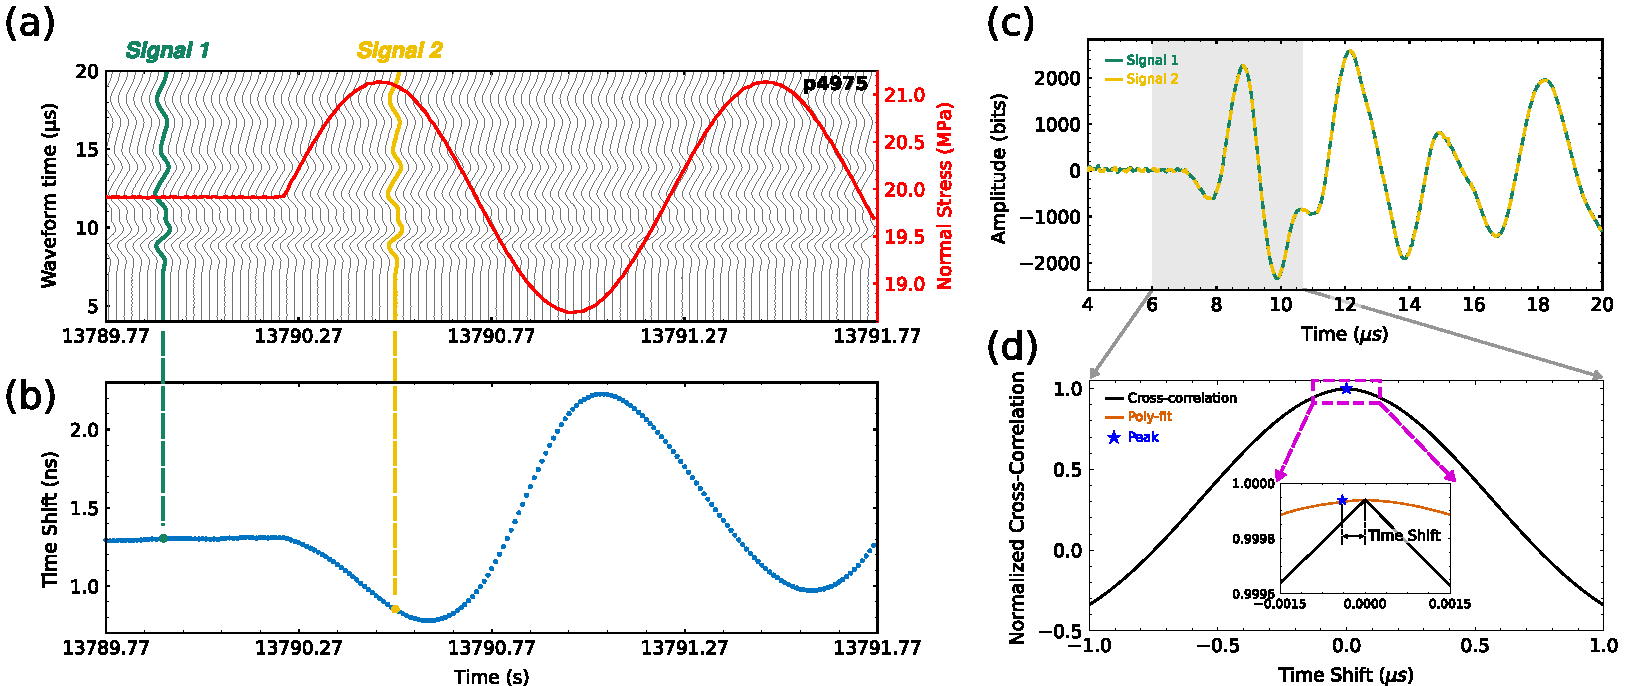
\includegraphics[width=0.9 \columnwidth]{xcor_fig_v3}
	\caption[]{(a) Excerpt from run4 of experiment p4966 shows part of a 1 Hz, 1 MPa normal stress oscillation (red) and the concurrent raw ultrasonic waveforms (grey). The number of waveforms in the waterfall plot has been decimated version for clarity. (b) Time shift was calculated by cross-correlating the waveforms to a reference waveform. (c) An example of a reference, unperturbed, waveform (green) and perturbed waveform (dashed yellow) highlights
		the similarity. (d) The maximum linear correlation between the reference and perturbed waveforms from cross-correlation is used to determine the time shift. The inset shows improvement of time shift calculations with a 2nd order polynomial fitting procedure.}
	\label{fig:xcor_poly}
\end{figure*}

\newpage